\chapter{Lagrangian Domain: Vortex Particle Method}
\label{ch:theory}

	
	\lsymb[f]{$\mathbf{x}$}{Position vector}{$[m]$}{x}
	\lsymb[f]{$\mathbf{x}_p$}{Position vector of the particle}{$[m]$}{xp}
	\lsymb[f]{$t$}{Time}{$[s]$}{t}
	\lsymb[f]{$\mathbf{u}$}{Velocity}{$[m\cdot s^{-1}]$}{u}
	%\lsymb[f]{$\mathbf{u}\left(\mathbf{x},t\right)$}{Velocity field}{$[m\cdot s^{-1}]$}{ua}
	\lsymb[f]{$p$}{Pressure}{$[\mathrm{Pa}]$}{p}
	\lsymb[f]{$\mathbf{u}^h$}{Discrete velocity}{$[m\cdot s^{-1}]$}{uh}	
	\lsymb[f]{$\mathbf{u}_{\infty}$}{Free-stream velocity}{$[m\cdot s^{-1}]$}{ul}
	\lsymb[f]{$\mathbf{u}_{\omega}$}{Vortical velocity}{$[m\cdot s^{-1}]$}{uz}
	\lsymb[f]{$\mathbf{u}_{\phi}$}{Potential velocity}{$[m\cdot s^{-1}]$}{up}
	\lsymb[f]{$N_p$}{Number of particles}{$[-]$}{np}	
	\lsymb[f]{$\mathbf{K}$}{Biot-Savart kernel}{[$-$]}{k}
	\lsymb[f]{$\mathbf{K_{\sigma}}$}{Vortex blob kernel}{[$-$]}{kb}	
	\lsymb[f]{$h$}{Nominal particle spacing}{[$m$]}{h}	
	\lsymb[f]{$\mathrm{overlap}$}{Overlap ratio of the blobs}{[$-$]}{o}	

	\gsymb[f]{$\zeta_{\sigma}$}{Smooth cut-off function of the blob}{[$-$]}{ff}	
	\gsymb[f]{$\rho$}{Density}{$[kg\cdot m^{-3}]$}{qq}
	\gsymb[f]{$\nu$}{Kinematic viscosity}{$[m^2\cdot s^{-1}]$}{mm}
	\gsymb[f]{$\Gamma$}{Circulation}{$[m^2\cdot s^{-1}]$}{g}
	\gsymb[f]{$\omega$}{Vorticity}{$[s^{-1}]$}{xx}
	\gsymb[f]{$\omega^h$}{Discrete vorticity field}{$[s^{-1}]$}{xx}
	\gsymb[f]{$\alpha_p$}{Circulation of the particle}{$[m^2\cdot s^{-1}]$}{ap}
	\gsymb[f]{$\sigma$}{Core size}{[$m$]}{rr}
	
	


%To model the flow around a VAWT, several approaches can be taken, Vermeer at al. (2003) \cite{Vermeer2003} have also summarized in their paper. The two main approaches of investigating the flow is either employing a numerical method to simulate the flow or through experimental simulations.

%Leishman (2006) \cite{leishman2006principles} has shown that there are several simplified, efficient numerical tools that can be used to model the performance of a VAWT. Methods such as actuator disk theory and blade element momentum theory and deals with simplified Navier-Stokes equations and is very useful to evaluate the trend of certain design parameter. However, as they are highly simplified, complex flow phenomenons that has severe impact of the performance characteristics of the VAWT such as flow separation during dynamic stall, vortex shedding during the rotation and blade-wake interaction cannot be simulated. In order to understand them, either experimental investigation such as in wind tunnel or full Navier-Stokes simulations have to undertaken. So to understand the flow behaviour of a VAWT, several numerical research have been performed \cite{Almohammadi2013} \cite{Ferreira2007} \cite{Islam2008} \cite{Merz2012} and experimental researches by Ferreira \cite{SimaoFerreira2008} \cite{Ferreira} and others \cite{Howell2010} \cite{Mertens2003}.
%\index{Actuator disk}

%All the numerical method that was grid-based struggled with dealing with large number of mesh cells for high Reynolds numbers and the numerical method that employed simplified Navier-Stokes methods had to sacrifices some accuracies.The experimental investigation also come with drawbacks as they are require more financial resources and usually only feasible to model the scaled VAWTs.

%This is the main relevance of the hybrid vortex particle method for the VAWT investigations. By utilizing the two methods together, the vortex particle method away from body, and Navier-Stokes solver with turbulence model in the near-body region, one will be able to tackle the challenges in an efficient manner.

%Therefore, this chapter is dedicated to given an overview on the theory of the Vortex Particle Method which we will employ with coupled Navier-Stokes solver. 

%------------------------------------------------------------------------------------------------------
%------------------------------------------------------------------------------------------------------
%------------------------------------------------------------------------------------------------------
\section{Introduction to Vortex Particle Method}
\printAcron{Vortex Particle Method}{VPM} is a branch of computational fluid dynamics that deals with the evolution of the vorticity of the fluid in a lagrangian description. Typically, the fluid is viewed at a fixed window where it is described as a function of space $\mathbf{x}$ and time $t$. However, the lagrangian point of view regards the fluid as a collection of the particles carrying the property of the fluid. 

%\todo{Lagrangian vs. Eulerian fluid diagram}

Unlike the typical eulerian method that require discretization of all the fluid domain, VPM only needs fluid elements where there is vorticity. This means that the VPM are inherently auto-adaptive method that only simulated the flow of interest. Furthermore, with the computational acceleration methods such as \printAcron{Fast-Multipole Method}{FMM} and parallel computation on \printAcron{Graphics Processing Units}{GPU}, VPM can be more efficient that typical eulerian methods.

\subsection{Vorticity}
Vorticity $\omega$, the governing element of vortex particle method, is defined as

	\begin{equation}
	\mathbf{\omega} = \Delta \times \mathbf{u},
	\end{equation}

where $\mathbf{u}$ is the velocity. The circulation $\Gamma$ is defined as

	\begin{equation}
	\Gamma = \int_L\mathbf{u}\cdot d \mathbf{r}=\int_S\omega\cdot\mathbf{n}\ dS,
	\label{eq:definitionOfCirculation}
	\end{equation}

by the stokes theorem, as represents the integral vorticity of the domain, figure \ref{fig:vorticityCirculation}

	\begin{figure}[t]
	\centering
	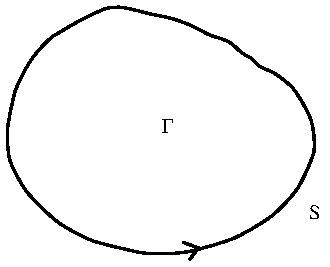
\includegraphics[width=0.3\linewidth]{./figures/lagrangian/vorticityCirculation.pdf}
	\caption{Circulation of the fluid}
	\label{fig:vorticityCirculation}
	\end{figure}

 
\subsection{Velocity-vorticity formulation of the Navier-Stokes equations}
The governing equation of the vortex particle method is velocity-vorticity $\mathbf{u}-\omega$ formulation of the Navier-Stokes equations \cite{Cottet2000a}. The 2-D incompressible Navier-Stokes momentum equation is given as

	\begin{equation}
	\frac{\partial \mathbf{u}}{\partial t} + \mathbf{u}\cdot\nabla\mathbf{u} = - \frac{1}{\rho} \nabla p + \nu \nabla^2\mathbf{u},
	\label{eq:mom}
	\end{equation}

relating the velocity field $\mathbf{u}\left(\mathbf{x},t\right)$ to the pressure field $\mathbf{p\left(\mathbf{x},t\right)}$, the kinematic viscosity $\nu$ and density $\rho$. Furthermore, we also have to satisfy the incompressibility constraint given as

	\begin{equation}
	\nabla\cdot\mathbf{u} = 0.
	\end{equation}

To attain the velocity-vorticity formulation, we should take the curl of the velocity-pressure $\mathbf{u}-p$ formulation of the Navier-Stokes equation. Taking the curl of the momentum equation \ref{eq:mom}, we get the vorticity transport equation

	\begin{equation}
	\frac{\partial \omega}{\partial t} + \mathbf{u}\cdot\nabla\omega = \nu \nabla^2 \omega,
	\end{equation}

which only relates the vorticity to the velocity enabling us to neglect the pressure field. Note that as we are dealing with the two dimensional flow, we neglected the stretching term. 


\subsection{Viscous splitting algorithm}
Vortex particle method was initially used to model the evolution of incompressible, inviscid flows. However, in order to simulate a real flow, we must also deal with the viscous behaviour of the fluid. Chorin \cite{Chorin1973} has shown that using the viscous splitting algorithm, it is possible to simulate a viscous flow. 

The viscous splitting algorithm is basically a fractional step method, where the viscous and the inviscid part of the transport equation is dealt in two subsequent steps, 

	\begin{itemize}
	\item Sub-step 1: convection
		\begin{equation}
		\frac{\partial\omega}{\partial t} + \mathbf{u}\cdot\nabla\omega=0;
		\label{eq:convectionEulerian}
		\end{equation}
		
	\item Sub-step 2: diffusion
		\begin{equation}
		\frac{\partial\omega}{\partial t} = \nu\nabla^2\omega.
		\end{equation}
	
	\end{itemize}

The first sub-step of the evolution deals with the convection of the vorticity. Note that, by convection we imply the advection of the vorticity field where the diffusion process is neglected. The second sub-step is where we deals with the diffusion of the vorticity field. 

There are several advantage to this type of evolution. As the convection and diffusion are handled separately, there is minimum dispersion during the convection and furthermore, the is no restriction of the advection CFL number \cite{Wee2006}.

There are many ways of dealing with the diffusion of the vorticity field. During this project, we use a modified interpolation kernel \cite{Wee2006} that can simultaneously treat diffusion and remesh the vortex particles, see section \ref{sec:diffusionVM}.

%------------------------------------------------------------------------------------------------------
%------------------------------------------------------------------------------------------------------
%------------------------------------------------------------------------------------------------------
\section{Spatial Discretization: Generation of Vortex Blobs}


In order to deal with the vorticity field, we must first discretize the vorticity to vortex particles. Vortex blobs have been first introduced by Chorin and is a mollified particle carrying the local circulation. Vortex blobs describes a smooth vorticity field and are ideal because of it does not cause singularity issues when particles approach each other.

\todo{check for consistency, continuity}
\subsection{Biot-Savart law}

The velocity field can be decomposed using the Helmholtz decomposition, given as

	\begin{equation}
	\mathbf{u} = \mathbf{u}_{\omega} + \mathbf{u}_{\phi},
	\end{equation}

where $\mathbf{u}_{\omega}$ is the rotational component of the velocity and $\mathbf{u}_{\phi}$ is the irrotational component. solenoidal and potential velocity respectively. In an unbounded flow we have $\mathbf{u}_{\phi}$ equal to the free-stream velocity $\mathbf{u}_{\infty}$. For bounded flow, we must include the presence of the body, see section \ref{sec:boundaryConditions}.
	
The velocity can be related to the vorticity using the Biot-Savart law

	\begin{equation}
	\mathbf{u}_{\omega} = \mathbf{K}\star\omega,
	\end{equation}
	
where the $\star$ represents convolution of the 2-D kernel $\mathbf{K}$ given by

	\begin{equation}
	\mathbf{K} = \frac{1}{2\pi\left|\mathbf{x}\right|^2}\left(-x_2,x_1\right).
	\label{eq:GreensKernel}
	\end{equation}
	
\subsection{Discrete form of vorticity field}
The spatial discretization of the fluid domain is done through $N$ quadrature points. With the Biot-Savart law, we can treat these quadratures are discrete particles carrying the local quantities. The discrete vorticity field is given as

	\begin{equation}
	\omega\left(\mathbf{x},t\right) \simeq \omega^h\left(\mathbf{x},t\right) = \sum_{p}\alpha_p\left(t\right)\delta \left[\mathbf{x}-\mathbf{x}_p\left(t\right)\right],
	\end{equation}

where $\alpha_{p}$ is the estimate of the circulation around the particle $\mathbf{x}_p$ with core size $\sigma$. We must not that $\omega^h$ is an approximately equal to $\omega$ of the fluid due to the discretization.

The discrete form of the velocity is therefore written as

	\begin{equation}
	\mathbf{u} \simeq \mathbf{u}^h = \sum_p \mathbf{K}\left[\mathbf{x}-\mathbf{x}_p\left(t\right)\right]\alpha_p\left(t\right).
	\end{equation}
	
Thus the discrete vorticity field is an $N$-body problem inducing velocity on each and implicitly evolving the vorticity field. This is one of the advantage of the vortex particle method as there are many ways to efficiently treat the problem. The $N$-body problem can be parallelized and can be accelerated using fast summation methods such as FMM, see \ref{sec:sat}.
	
However, like all $N$-body problem, equation \ref{eq:GreensKernel} has a singularity when the particles approach each other and can result in numerical instability. To overcome this we can mollify the kernel, removing the singularity.

\subsection{Convection of vortex blobs}

In the discrete of the convection equation \ref{eq:convectionEulerian} of the viscous-splitting algorithm, the is solved as system of ODEs, where

	\begin{equation}
	\frac{\mathrm{d}\mathbf{x}_p}{\mathrm{d}t} = \mathbf{u}\left(\mathbf{x}_p\right),
	\end{equation}
with
	\begin{equation}
	\frac{\mathrm{d}\Gamma_p}{\mathrm{d}t} = 0.
	\end{equation}

As the diffusion is done at the next sub-step, we have to ensure that the circulation is conserved.


\subsection{Mollified vortex kernels}

A vortex particle with a mollified core, non-zero core-size, is referred to as vortex blobs. The advantage of the vortex blobs is that the with a smooth distribution of the vorticity, the singularity disappears and so numerical instability does not happen when blobs get too close to each other. An ideal choice for a cutoff function is a Gaussian distribution, figure \ref{fig:gaussianDistribution}.

	\begin{figure}[t]
	\centering
	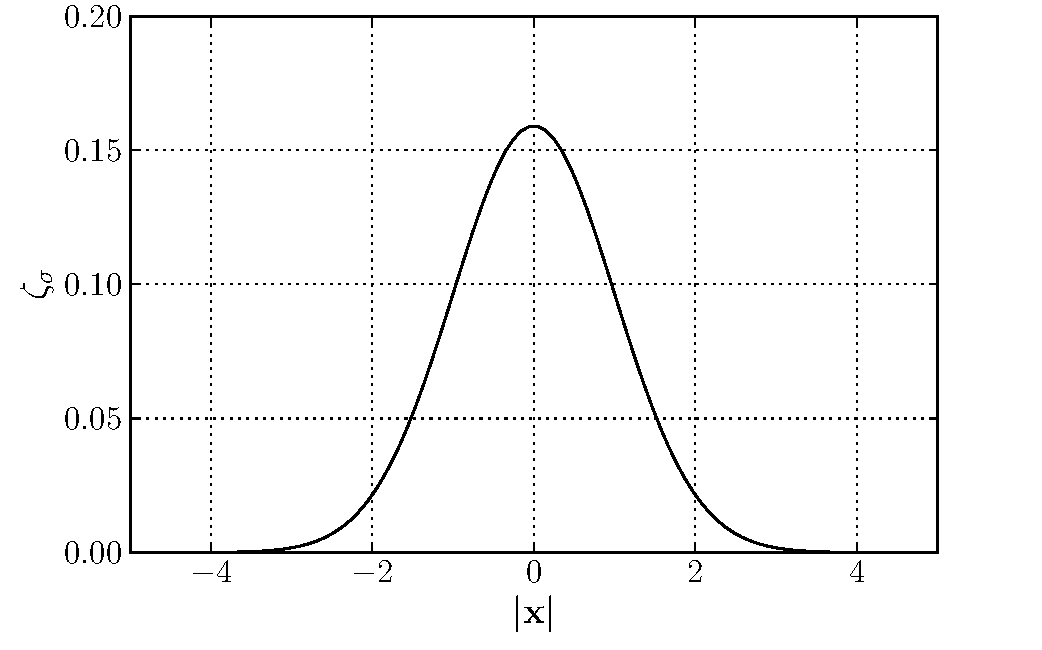
\includegraphics[width=0.7\textwidth]{figures/lagrangian/gaussianKernel.pdf}
	\caption{Vortex blob with Gaussian distribution: [$k=2$, $\sigma=1.0$]}
	\label{fig:gaussianDistribution}
	\end{figure}

Gaussian kernels satisfy the requirement for smooth distribution ad decays quickly and is defined as
	
	\begin{equation}
	\zeta_{\sigma} = \frac{1}{k\pi\sigma^2}\exp\left(\frac{-\left|\mathbf{x}\right|}{k\sigma^2}\right),
	\end{equation}

where $k$ is 1, 2 or 4 and determines the width of the kernel, $\sigma$ is core-size of the blob. Note that smoothing function is chosen such that $\int \zeta = 1$, ensuring the conservation of circulation when mollified. So, using a smooth cut-off function $\zeta_{\sigma}$, the mollified kernel $\mathbf{K}_{\sigma}$ is given as 

	\begin{equation}
	\mathbf{K}_{\sigma} = \mathbf{K} \star \zeta_{\sigma}.
	\end{equation}

The mollified vorticity field, represented by vortex blobs is given as

	\begin{equation}
	\omega^h\left(\mathbf{x},t\right) = \sum_p \alpha_p\left(t\right)\zeta_{\sigma}\left[\mathbf{x}-\mathbf{x}_p\left(t\right)\right],
	\label{eq:mollifiedVorticityField}
	\end{equation}

now representing the mollified vorticity field and equivalently, the mollified velocity field is given as

	\begin{equation}
	\mathbf{u}^h\left(\mathbf{x},t\right) = \sum_p \mathbf{K}_{\sigma}\left[\mathbf{x}-\mathbf{x}_p\left(t\right)\right]\alpha_p\left(t\right).
	\end{equation}

Koumoutsakos and Chorin \cite{Cottet2000a}, have shown that for proper communication between the particle, the particle needs to overlap,

	\begin{equation}
	\mathrm{overlap} = \frac{\sigma}{h},
	\end{equation}

	\begin{figure}[b]
	\centering
	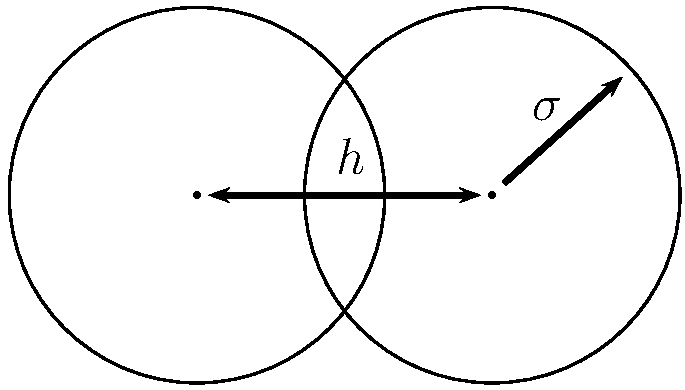
\includegraphics[width=0.4\textwidth]{figures/lagrangian/blobOverlap.pdf}
	\caption{Vortex blob with overlap $\sigma/h$}
	\label{fig:blobOverlap}
	\end{figure}

	
where $h$ is the nominal particle spacing, figure \ref{fig:blobOverlap}. If the particles fail to overlap, vortex blobs will also fail to recover the vorticity field. Such problems occurs when blobs are clustered due to high flow strain, leading to lagrangian grid distorting and must be treated, see section \ref{subsec:remeshing}.


\subsection{Vortex blob initialization}

Now the question arises on how to initialize the particle's circulation strengths $\alpha_p$. A common approach that is used is to estimate the particles strength is to say that

	\begin{equation}
	\alpha_p = \omega_p\cdot h^2.
	\label{eq:particleCirculationAssignment}
	\end{equation}

This might seem like a valid assumption as the circulation of a given area is the integral of the vorticity in the area, equation \ref{eq:definitionOfCirculation}, however this is no longer valid when regularizing the vorticity field using mollified gaussian kernels, equation \ref{eq:mollifiedVorticityField}. Barba and Rossi \cite{Barba2010}, has described this problem as gaussian blurring of the original vorticity field. Even though the particle have acquired the correct circulation strengths (i.e the local property), when evaluating the mollified vorticity field, we see that there is a mismatch in the evaluated vorticity field, figure \ref{fig:particleInitialization}. 


	\begin{figure}[t]
	\centering
	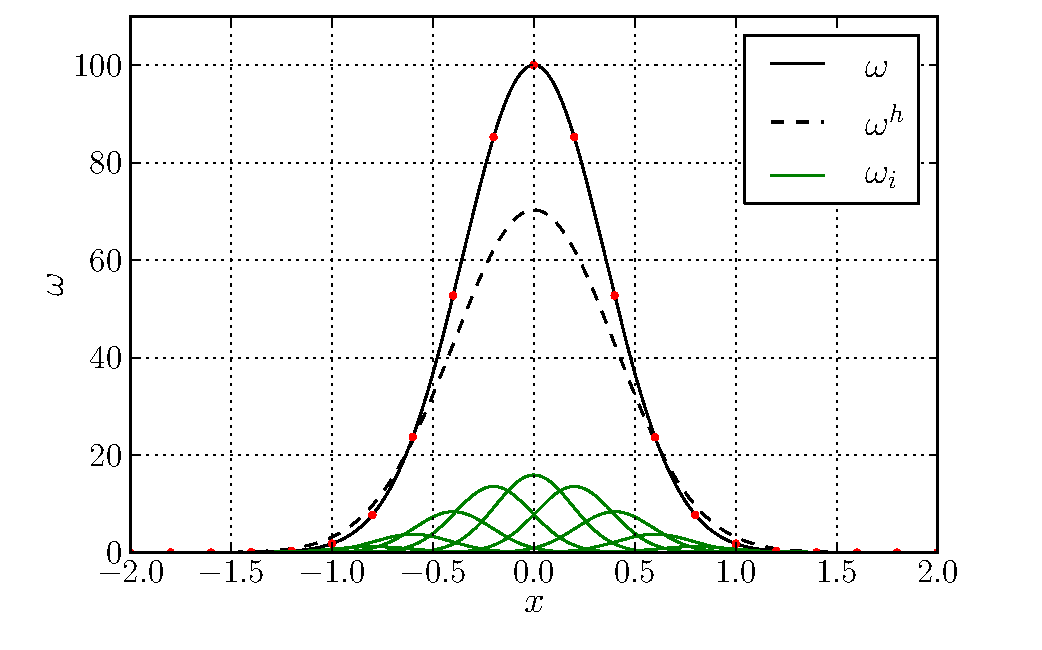
\includegraphics[width=0.7\textwidth]{figures/lagrangian/particleInitialization.pdf}
	\caption{Mollified vorticity field of an arbitrary vorticity function with $\mathrm{overlap}=1.0$, $\sigma=0.19$, $h=0.19$. Vortex blob strength has been assigned by equation \ref{eq:particleCirculationAssignment}, sampling at exact vorticity [{\color{plotRed}{$\bullet$}}, red dot]. Figure depicts exact vorticity distribution $\omega$ [---, solid], vorticity field of each blob $\omega_i$ [{\color{darkgreen}{---}}, green dashed], the mollified vorticity field $\omega^h$ [- -, dashed].  }
	\label{fig:particleInitialization}
	\end{figure}

Another way of viewing this characteristic is say the conservation of circulation is only valid globally, but not locally. A common standard for recovering the initial vorticity field is perform the Beale's method \cite{Beale1988}.

\subsubsection*{Beale's Iterative Method}

The Beale's method is particle circulation processing scheme where the circulation of the particles are modified such that the mollified vorticity field matches the indented vorticity field. The recovery of the vorticity field is done by performing a discrete deconvolution,

	\begin{equation}
	\sum_j^N \beta_j \zeta_{\sigma}\left(\mathbf{x}_i-\mathbf{x}_j\right) = \omega_i,
		\end{equation}

where $\beta_j$ is the circulation of the particles at positions $\mathbf{x}_j$ such that it matches the exact vorticity $\omega_i$ at the position $\mathbf{x}_i$ that we are evaluating.  As we are try to solve for a $N$ unknown problem, we must set up a $N$ system of equations. Multiplying both sides with the area associated to the blobs, we get

	\begin{equation}
	\mathbf{A}_{ij} \beta_j = \alpha_i^{\mathrm{exact}},
	\end{equation}
	
where

	\begin{equation}
	\mathbf{A}_{ij} = \zeta_{\sigma}\left(\mathbf{x}_i - \mathbf{x}_j\right) \cdot h^2
	\end{equation}

is a $N \times N$ matrix containing the weights of the influence of each particle on each other. This matrix can be constructed by setting the $\Gamma$ to one and determine the induced vorticity on each other. Furthermore, we see that it is not feasible to directly invert the matrix when we have large set of blobs but most importantly as the matrix $\mathbf{A}$ is severly ill-conditioned \cite{Speck2011a}, it should not be directly inverted. Beale's proposition to this problem was to iteratively solve for the solution,

	\begin{equation}
	\beta_{j}^{n+1} = \alpha_i + \beta_i^n - \mathbf{A}_{ij}\cdot\beta_j^n
	\end{equation}
	
We see that with just two iterations, the error between the mollified and exact vorticity field reduces drastically, figure \ref{fig:bealesCorrection}. Koumoutsakos and Cottet \cite{Cottet2000a}, had shown that there was a drastic improvement in the velocity with just two to three iterations. However, we see that the cell vorticity of the blobs, directly evaluated from the particle strengths, equation \ref{eq:particleCirculationAssignment}, are more peaky and no longer matches the exact vorticity. 

During the hybrid coupling algorithm, we see that this is the central source of coupling error between the eulerian and the lagrangian method, section \ref{}. When performing the hybrid coupling, we need to recover the vorticity field transfered from the eulerian domain to the lagrangian domain in every step. So, beale's correction is not a viable solution for the hybrid method. Thus there is a need for an alternate method of recovering the vorticity field.

\todo{add the reference to hybrid}

	\begin{figure}[t]
	\centering
	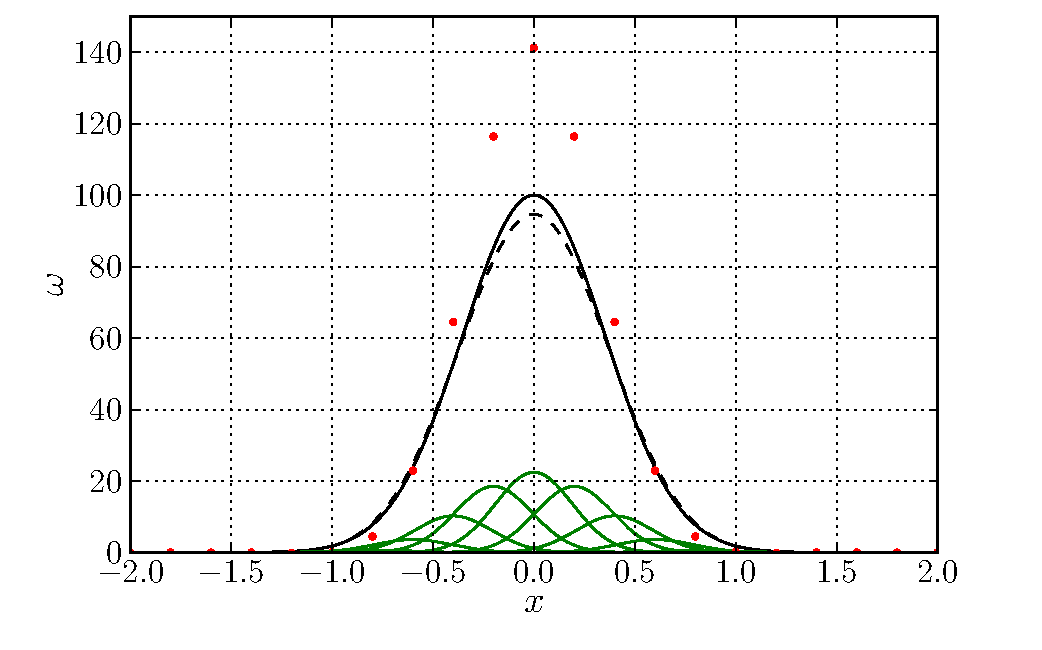
\includegraphics[width=0.7\textwidth]{figures/lagrangian/bealesCorrection.pdf}
	\caption{Mollified vorticity field after two Beale's iteration, $\mathrm{overlap}=1.0$, $\sigma=0.19$, $h=0.19$. Figure depicts exact vorticity distribution $\omega$ [---, solid], vorticity field of each blob $\omega_i$ [{\color{plotGreen}{---}}, green dashed], the mollified vorticity field $\omega^h$ [- -, dashed].  }
	\label{fig:bealesCorrection}
	\end{figure}



\subsubsection{Convergence of particle discretization}

An alternate, temporary method to reduce the gaussian blurring of the vorticity field is to reduce the overlap (i.e. increase the overlap ratio) of the vortex blobs and to the increase the spatial resolution.
	
\begin{figure}[b]
        \centering
        \begin{subfigure}[b]{0.5\textwidth}
                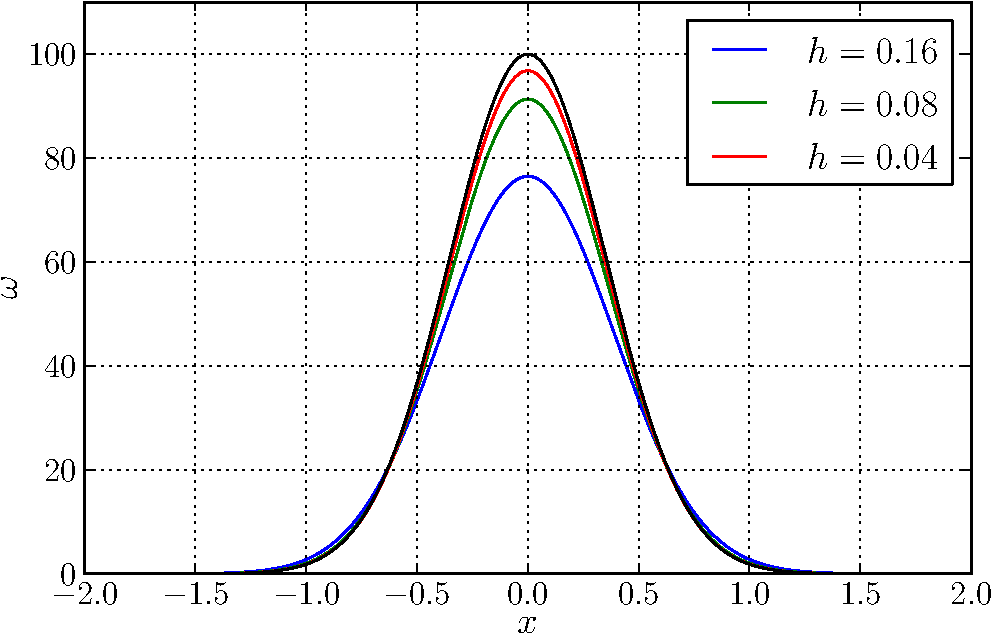
\includegraphics[width=\textwidth]{figures/lagrangian/betterInitialization_h-crop.pdf}
                \caption{Convergence of $h$ with $\mathrm{overlap} = 1.0$}
                \label{fig:convergenceOfBlobsH}
        \end{subfigure}%
        ~ %add desired spacing between images, e. g. ~, \quad, \qquad etc.
          %(or a blank line to force the subfigure onto a new line)
        \begin{subfigure}[b]{0.5\textwidth}
                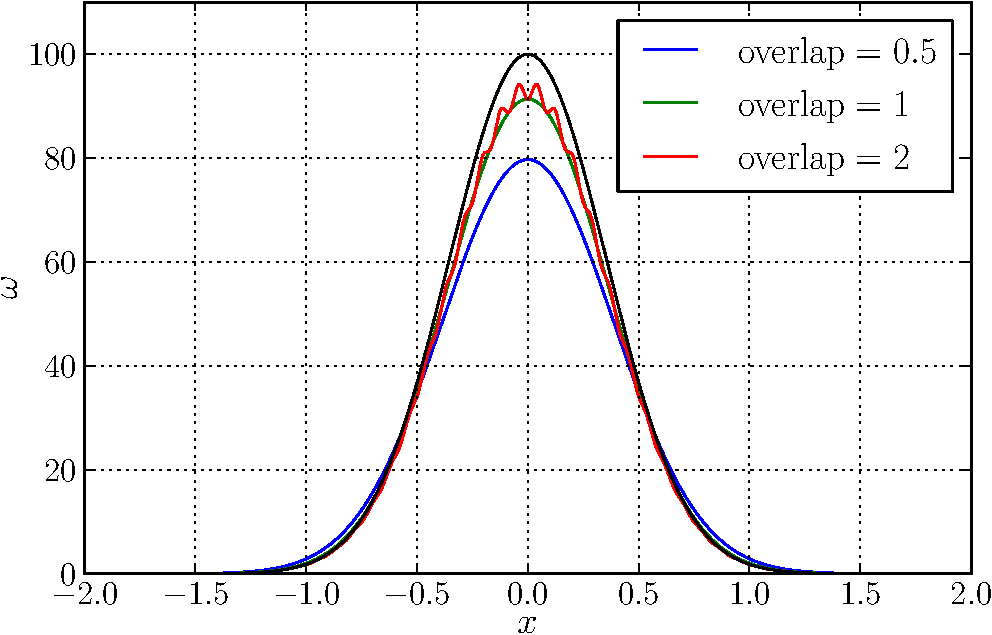
\includegraphics[width=\textwidth]{figures/lagrangian/betterInitialization_overlap-crop.pdf}
                \caption{Convergence of $\mathrm{overlap}$ with $h = 0.08$}
                \label{fig:convergenceOfBlobsOverlap}
        \end{subfigure}
        \caption{Convergence of vorticity by modifying the spatial resolution. Figure depicts exact vorticity field $\omega$ with [---, black] and various resolutions.}
        \label{fig:convergenceOfSpatialResolution}
\end{figure}	

Figure \ref{fig:convergenceOfSpatialResolution} shows mollified vorticity field results from modifying the spatial resolution parameters. Figure \ref{fig:convergenceOfBlobsH} shows the convergence of the mollified vorticity field $\omega^h$ to the exact vorticity field $\omega$ by reducing the nominal particle spacing $h$. The blobs have $\mathrm{overlap} = 1$ and so the blob core-size $\sigma$ is equal to $h$. We see that as you reduce the size of the blob and increase the number of particles, the mollified vorticity converges to the exact vorticity. Therefore, an alternate method of reducing the gaussian blurring is to increase the spatial resolution.

Furthermore, we could also adjust the $\mathrm{overlap}$ of the blobs, figure \ref{fig:convergenceOfBlobsOverlap}. The $\sigma$ and $h$ of the blob is $0.08$ and we see that increasing overlap number (i.e reducing the overlap), helps us to recover the original vorticity field. However, as explained by Koumoutsakos \cite{Cottet2000a}, if the overlap is too low, we lose the smooth recovery of the vorticity field. This is apparent when $\mathrm{overlap} = 2.0$, where we see that the mollified vorticity field is fluctuation.

Therefore, for the hybrid coupling, we set $\mathrm{overlap} = 1.0$ and maximize the spatial resolution at the coupling zone. 

\subsection{Remeshing scheme: Treating lagrangian grid distortion}
\label{subsec:remeshing}
%
%%------------------------------------------------------------------------------------------------------
%%------------------------------------------------------------------------------------------------------
%%------------------------------------------------------------------------------------------------------

During the convection step, we see that another source of error in the vorticity field is the lagrangian grid distortion. As we have seen before, when the vortex blobs fails to overlap, we are no longer able to reconstruct the correct the vorticity field, figure \ref{fig:convergenceOfBlobsOverlap}. During the convection, due to the high strains in the fluid, the vortex blobs tent to clump together and creates regions where no vortex blobs are found, reducing the overlap of the blobs, figure \ref{fig:distortion}. 

%\begin{figure}[t]
%        \centering
%        \begin{subfigure}[b]{0.45\textwidth}
%                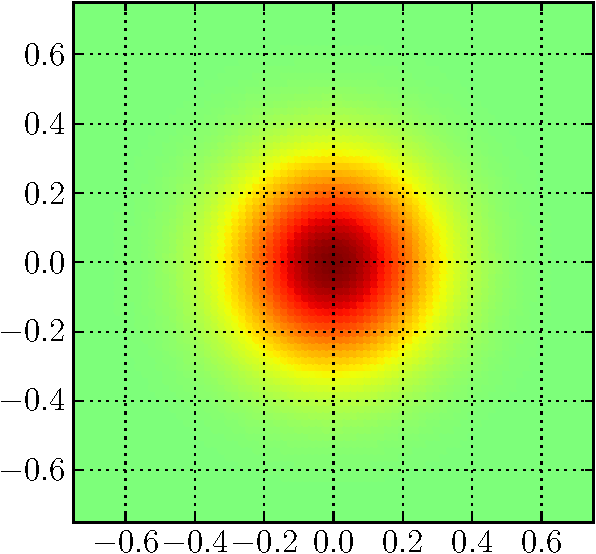
\includegraphics[width=\textwidth]{figures/lagrangian/distortion_a-crop.pdf}
%                \caption{$t = 0$}
%                \label{fig:distortion_a}
%        \end{subfigure}%
%        \qquad %add desired spacing between images, e. g. ~, \quad, \qquad etc.
%          %(or a blank line to force the subfigure onto a new line)
%        \begin{subfigure}[b]{0.45\textwidth}
%                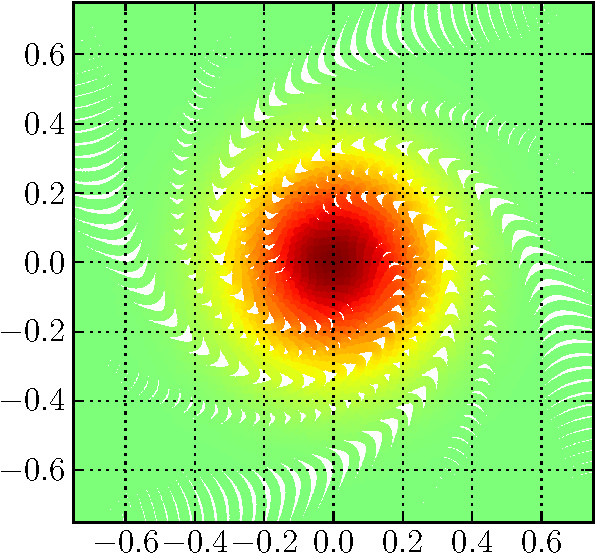
\includegraphics[width=\textwidth]{figures/lagrangian/distortion_b-crop.pdf}
%                \caption{$t = 10$}
%                \label{fig:distortion_b}
%        \end{subfigure}
%        \caption{Lagrangian distortion of the vortex blobs after 100 steps. The initial vorticity field $\omega\left(\mathbf{x},0\right) = \exp\left(-12\left|\mathbf{x}\right|\right)$ with $\Delta t = 0.1$, $\sigma=0.02$ and $\mathrm{overlap} = 1.0$. Figure depicts the initial and the final distribution of the vortex blobs.}
%        \label{fig:distortion}
%\end{figure}

	\begin{figure}[t]
	\centering
	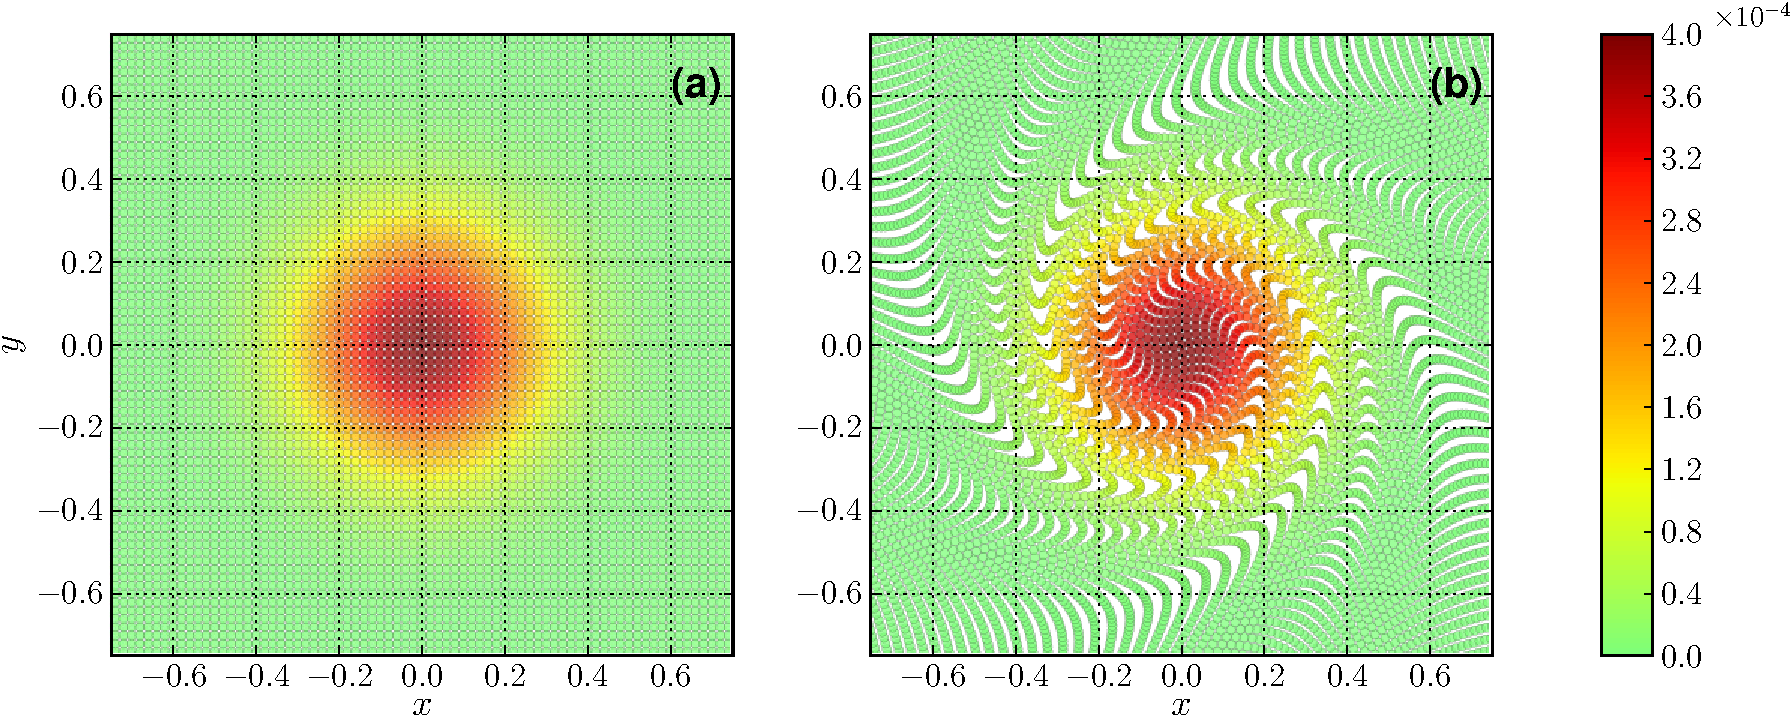
\includegraphics[width=0.9\textwidth]{figures/lagrangian/distortion-crop.pdf}
    \caption{Lagrangian distortion of the vortex blobs after 100 steps. The initial vorticity field $\omega\left(\mathbf{x},0\right) = \exp\left(-12\left|\mathbf{x}\right|\right)$ with $\Delta t = 0.1$, $\sigma=0.02$ and $\mathrm{overlap} = 1.0$. Figure depicts the initial and the final distribution of the vortex blobs.}
    \label{fig:distortion}
	\end{figure}


We see that due to clustering of the vortex blobs, it fails to reproduce the correct vorticity field. A common strategy to overcome this problem is to remesh the vortex blobs to a uniform grid, so that we have a continuous vorticity field.

However, when transfering the vorticity from the old deformed grid to the new lagrangian uniform grid, we must satisfy the conservation laws of vorticity field. The interpolation methods is based on the conservation of linear impulse which directly implies the conservation of the total circulation \cite{Cottet2000a}. The transfer of the particle strengths is given as, 

	\begin{equation}
	\alpha_p = \sum_q\tilde{\alpha}_q W \left(\frac{x_p - \tilde{x}_q}{h}\right),	
	\end{equation}

where the strengths of the particles $\tilde{\alpha}_q$ of the distorted lagrangian grid $\tilde{x}_q$ is transfered to the regular lagrangian grid $x_p$ using the interpolation kernel, weighted $W$, giving us the remeshing particle strengths $\alpha_p$. The transfer of strengths of one particles to it's interpolation nodes can be seen in figure \ref{fig:interpolationGrid}.


	\begin{figure}[t]
	\centering
	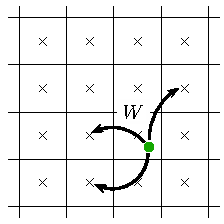
\includegraphics[width=0.4\textwidth]{figures/lagrangian/interpolationGrid.pdf}
	\caption{Interpolation of vortex blob ({\color{plotGreen}{$\bullet$}}, green) on the uniform grid.}
	\label{fig:interpolationGrid}
	\end{figure}

\subsubsection*{$\mathbf{M}^\prime_4$ interpolation kernel}
For lagrangian problem, we use the efficient interpolation kernel that has been used to reconstruct a smooth distribution interpolation, the $\mathrm{M}^{\prime}_4$ interpolation kernel, introduced by Monaghan \cite{Monaghan1985}. In one dimension it is given as,

	\begin{equation}
	{\mathrm{M'}_4}\left( {\xi} \right) =
	  \begin{cases}
	   {1 - \frac{{5{\xi ^2}}}{2} + \frac{{3{{\left| \xi  \right|}^3}}}{2}} & {\left| \xi \right|} < 1, \\
	   \frac{1}{2}{\left( {2 - \left| \xi  \right|} \right)^2}\left( {1 - \left| \xi  \right|} \right) & 1 \le {\left| \xi \right|} < 2,\\
	   0 & 2 \le \left| \xi \right|,
	  \end{cases}
	\label{eq:interpKernel}
	\end{equation}

where $\xi = x_p - x$ is the distance of the particle to the interpolation nodes. The $\mathrm{M'}_4$ is a third-order accurate piecewise smooth B-spline kernel, where $m = 4$ giving it 4 support nodes, figure \ref{fig:interpolationKernel}. For the two dimensional problem that we have, the 2-D interpolation formula is simply tensor product of the 1-D interpolation kernel equation \ref{eq:interpKernel}, and results in $4^2 = 16$ support nodes, figure \ref{fig:interpolationGrid}.

	\begin{figure}[t]
	\centering
	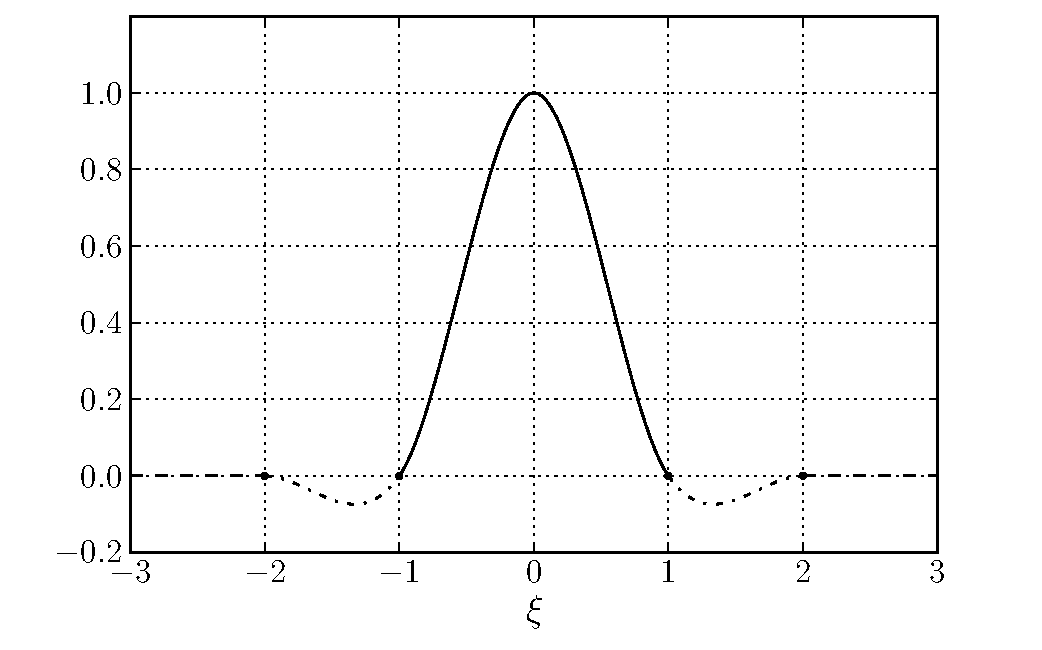
\includegraphics[width=0.7\textwidth]{figures/lagrangian/interpolationKernel.pdf}
	\caption{Interpolation kernel}
	\label{fig:interpolationKernel}
	\end{figure}

The interpolation kernel achieves the third-order accuracy as it also conserves the linear and the angular momentum of the vortex. Koumoutsakos \cite{Koumoutsakos1997} has investigated the drawback of the employing the remeshing strategy and have shown that there is approximately $4\%$ decay in enstrophy of the flow due to sub-grid dissipation. 

\section{Diffusion of Vortex Methods}
\label{sec:diffusionVM}

Chorin initially employed a random walk method, however this method suffers some limitations in accuracy and since then several methods have been introduced that can be used to simulate the diffusion. \printAcron{Particle Strength Exchange}{PSE} method \cite{Degond1989}, is an algorithm to treat diffusion by exchange of vortex element strengths. \printAcron{Vortex Redistribution Method}{VRM} \cite{Shankar1996} models diffusion by distributing the fraction of circulation of the vortex elements to the neighbouring vortices. 

\subsection{Vorticity diffusion techniques}
%
\subsection{Modified remeshing for treating diffusion}
The diffusion method that is applied here has been proposed by Shankar and Van Dommelen \cite{Shankar1996} and the modified ${{{\rm{M'}}}_4}$ interpolation kernel has been derived by Ghoniem and Wee \cite{Wee2006} and was also applied by Speck \cite{Speck2011}. The diffusion is simulated by the modified interpolation kernel during the remeshing process. During remeshing, the heat equation is satisfied by transferring the correct fraction of circulation to produce the proper amount of diffusion. The ${{{\rm{M'}}}_4}$ kernel was modified to treat the diffusion and is given by: 

\begin{equation}
{{{\rm{M'}}}_4}\left( {\xi ,c} \right) =
  \begin{cases}
   {1 - \frac{{5{\xi ^2}}}{2} + \frac{{3{{\left| \xi  \right|}^3}}}{2} - {c^2}\left( {2 - 9{\xi ^2} + 6{{\left| \xi  \right|}^3}} \right)} & {\left| \xi \right|} < 1, \\
   \frac{1}{2}{\left( {2 - \left| \xi  \right|} \right)^2}\left( {1 - \left| \xi  \right|} \right) - {c^2}{\left( {2 - \left| \xi  \right|} \right)^2}\left( {1 - 2\left| \xi  \right|} \right) & 1 \le {\left| \xi \right|} < 2,\\
   0 & 2 \le \left| \xi \right|,
  \end{cases}
\label{eq:modInterpKernel}
\end{equation}

where 

\begin{equation}
c^2 = \frac{\nu \Delta t_d}{h^2},
\label{eq:c2}
\end{equation}

and corresponds to the transfer quantity for diffusion. The $\nu$ denotes the viscosity of the fluid, $t_d$ is the diffusion time step and $\Delta x$ is the blob spacing. When $c \rightarrow 0$, the interpolation kernel turns to the classical non-diffusion kernel.  This modified interpolation kernel conserves the circulation of each vortex and also satisfies the conservation of linear and angular momentum of the vorticies.

The vortex method employs the viscous splitting procedure, where the vortex blobs are convected first and is then diffused through the remeshing process using the modified interpolation kernel. The advantage of this methodology is that the convection process is not constrained by the CFL condition. So, the convection time step size can be different than from the diffusion time step size and the diffusion time step size is a multiple of the convection time step size depending on the redistribution frequency $f_{redist}$. Therefore, the constrained that is imposed on the redistribution frequency is the stability bounds of the modified interpolation kernel. Analyzing the amplification factor and the phase error of the modified interpolation kernel in the Fourier space requires that the $c^2$ should be as follows:


\begin{equation}
\frac{1}{6} \le c^2 \le \frac{1}{2}.
\label{eq:c2stability}
\end{equation}

This will ensure the stability of the problem and will suppress any spurious oscillations and ensure that it is a non-negative interpolation kernel with non-negative redistribution fractions.

\subsection{Convergence study of the viscous vortex method}
%%------------------------------------------------------------------------------------------------------
%%------------------------------------------------------------------------------------------------------
%%------------------------------------------------------------------------------------------------------
\section{Boundary conditions at solid boundary}
\label{sec:boundaryConditions}

\subsection{Boundary integral equations}
%
\subsubsection{Linked boundary conditions}
%
\subsection{Panel method for treating no-slip boundary condition}
%
\subsection{Convergence study of panel method}
%
\section{Simulation acceleration techniques}
\label{sec:sat}
%
\subsection{Fast multi-pole Method}
%
\subsection{Parallel computation in GPU}
%
\section{Validation of lagrangian method}

\subsection{Lamb-oseen vortex at $Re=100$}
%
\subsection{Convection of Clercx-Bruneau dipole at $Re=625$}
%
\section{Summary}
%
